\chapter{Prototyp}
\label{Prototyp}
\nicetohave{Einleitung?}
Das Konzept beschreibt, welche Funktionen umgesetzt werden müssen und wie die Informationen für den Problemlöseprozess dargestellt werden können. In diesem Abschnitt wird das Konzept in das Design der PFE \cite{} \todo{Verweis} eingegliedert und anhand des Use Case prototypisch dargestellt.

Der Prototyp wird mit dem Programm Axure \cite{axure} \todo{Verweis} umgesetzt. Neben der Möglichkeit einen digitalen Prototypen umfangreich umzusetzen, bietet das Programm auch sehr gute Voraussetzungen für eine abschließende Validierung.
\\ \\
Während des Problemlöseprozesses nimmt das Systeme verschiedene Zustände an (siehe Abbildung \ref{pic:Zustandsdiagramm-Assistenzsystem}). Zu Beginn ist nur die grundlegende PFE dargestellt. Nach sieben Sekunden zeigt das System eine Meldung an, die durch das Modul Temper ausgelöst wurde. Nach Erscheinen der Meldung hat der Nutzer die Möglichkeit auf den Button \textbf{Problem bearbeiten} zu klicken. Durch diese Aktion wird das Problem genauer angezeigt. Die Interaktionsmöglichkeiten in diesem Zustand sind in Abschnitt \ref{5:Problembeschreibung} näher beschrieben. Nach der Begutachtung und Spezifikation des Problems wechselt das Assistenzsystem durch Betätigung des Buttons\textbf{ Lösungen finden}, abhängig von den eingegebenen Zielen, in den Zustand \textit{Lösungen}. Soll das Problem bearbeitet werden so kann in den Zustand \textit{Problem} durch Klicken auf \textbf{Problembeschreibung} gewechselt werden. 

\begin{figure}[tbp]
\centering
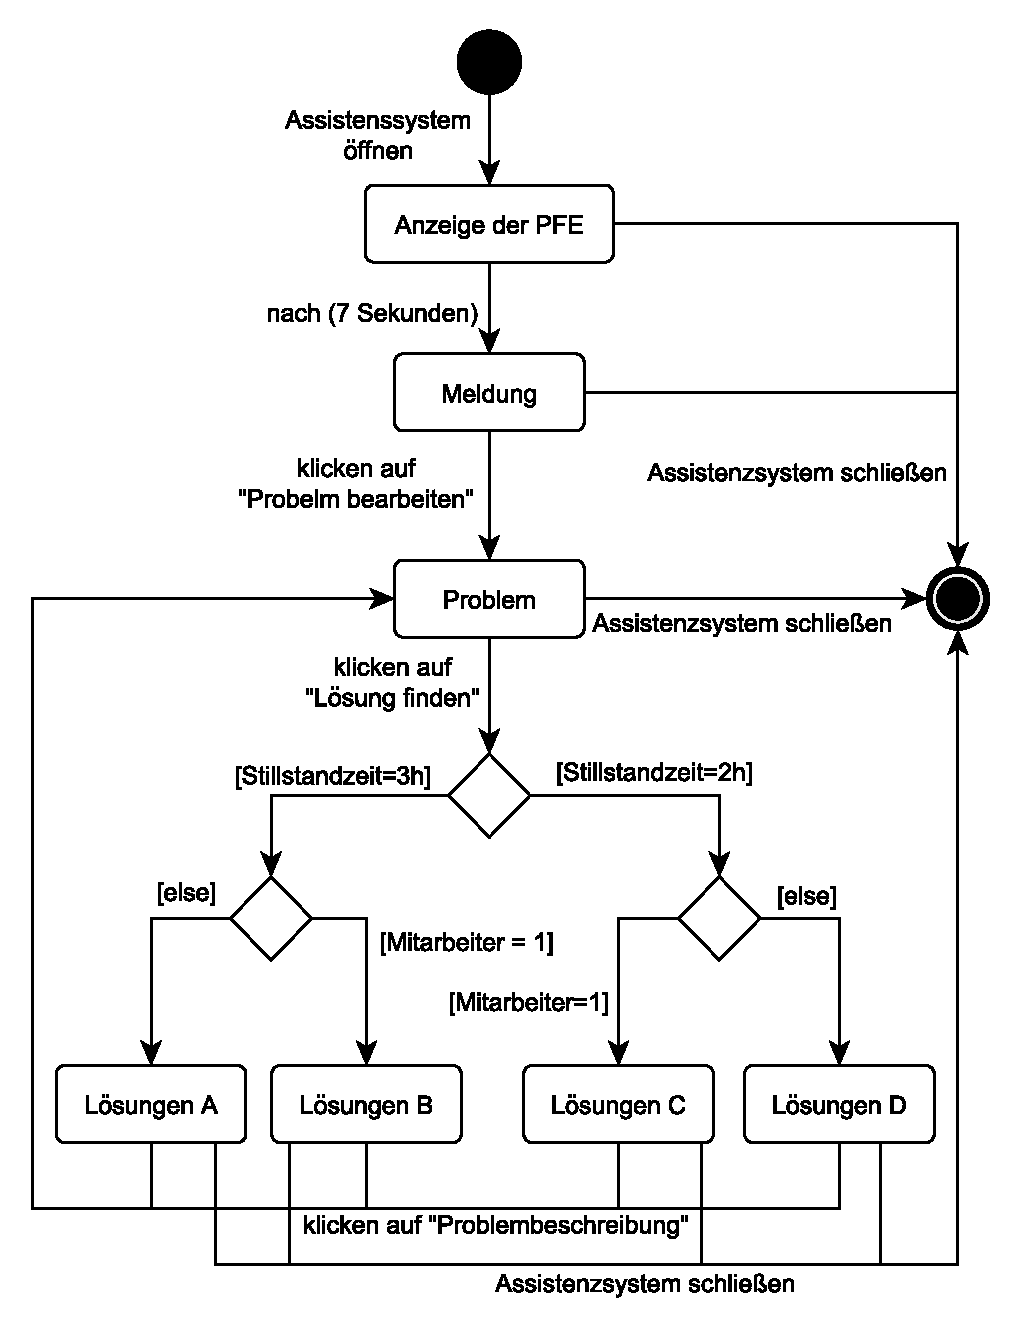
\includegraphics[scale=0.65]{DA_files/UML/Prototyp/Zustandsdiagramm-Assistenzsystem.pdf}
\caption{Zustandsdiagramm Assistenzsystem - Prototyp}
\label{pic:Zustandsdiagramm-Assistenzsystem}
\end{figure}

\section{Prozessführungsebene}
Da das Assistenzsystem in die bestehende Prozessführungsebene eingegliedert wird, müssen die grundlegenden Funktionalitäten dieser zunächst im Prototyp nachgebaut werden. Die grafischen Elemente liegen bereits in geeigneter Form vor und werden nur noch korrekt verknüpft. Dies umfasst zum einen die Elemente innerhalb der Bereiche (vgl. Abschnitt \ref{3:PFE}), als auch die Verknüpfungen zwischen den Bereichen.

\subsection{Navigation}
In der Navigation kann die Ansicht zwischen dem Shopfloor und der ausgewählten Subplant  gewechselt werden (siehe Abbildung \ref{pic:Zustandsdiagramm-Navigation}). Da die Veränderung des Zustands in der Navigation auch die Ansicht des Rezepts verändert, werden entsprechende Signale an das Rezept gesendet.
\begin{figure}[htbp]
\centering
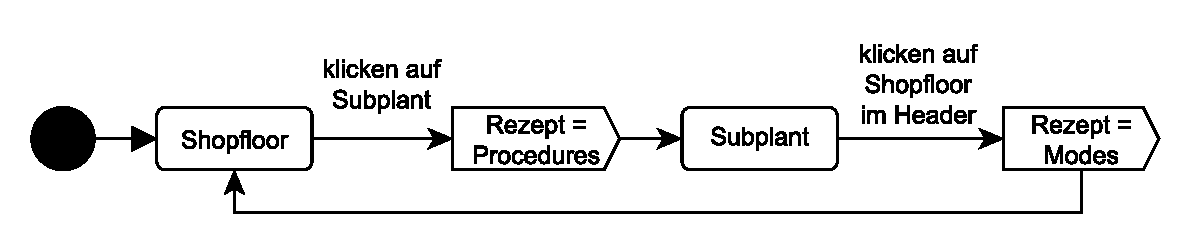
\includegraphics[scale=0.65]{DA_files/UML/Prototyp/Zustandsdiagramm-Navigation.pdf}
\caption{Zustandsdiagramm Navigation - Prototyp}
\label{pic:Zustandsdiagramm-Navigation}
\end{figure}

Zeigt die Navigation die Subplant an, kann der Nutzer durch Klicken ein Modul anwählen. Diese Auswahl hat Einfluss auf die Rezeptansicht und den Service Launcher. Die entsprechenden Aktionen des Systems sind in Abbildung \ref{pic:Aktivitaetsdiagramm-Navigation-Subplant} dargestellt.
\begin{figure}[htbp]
\centering
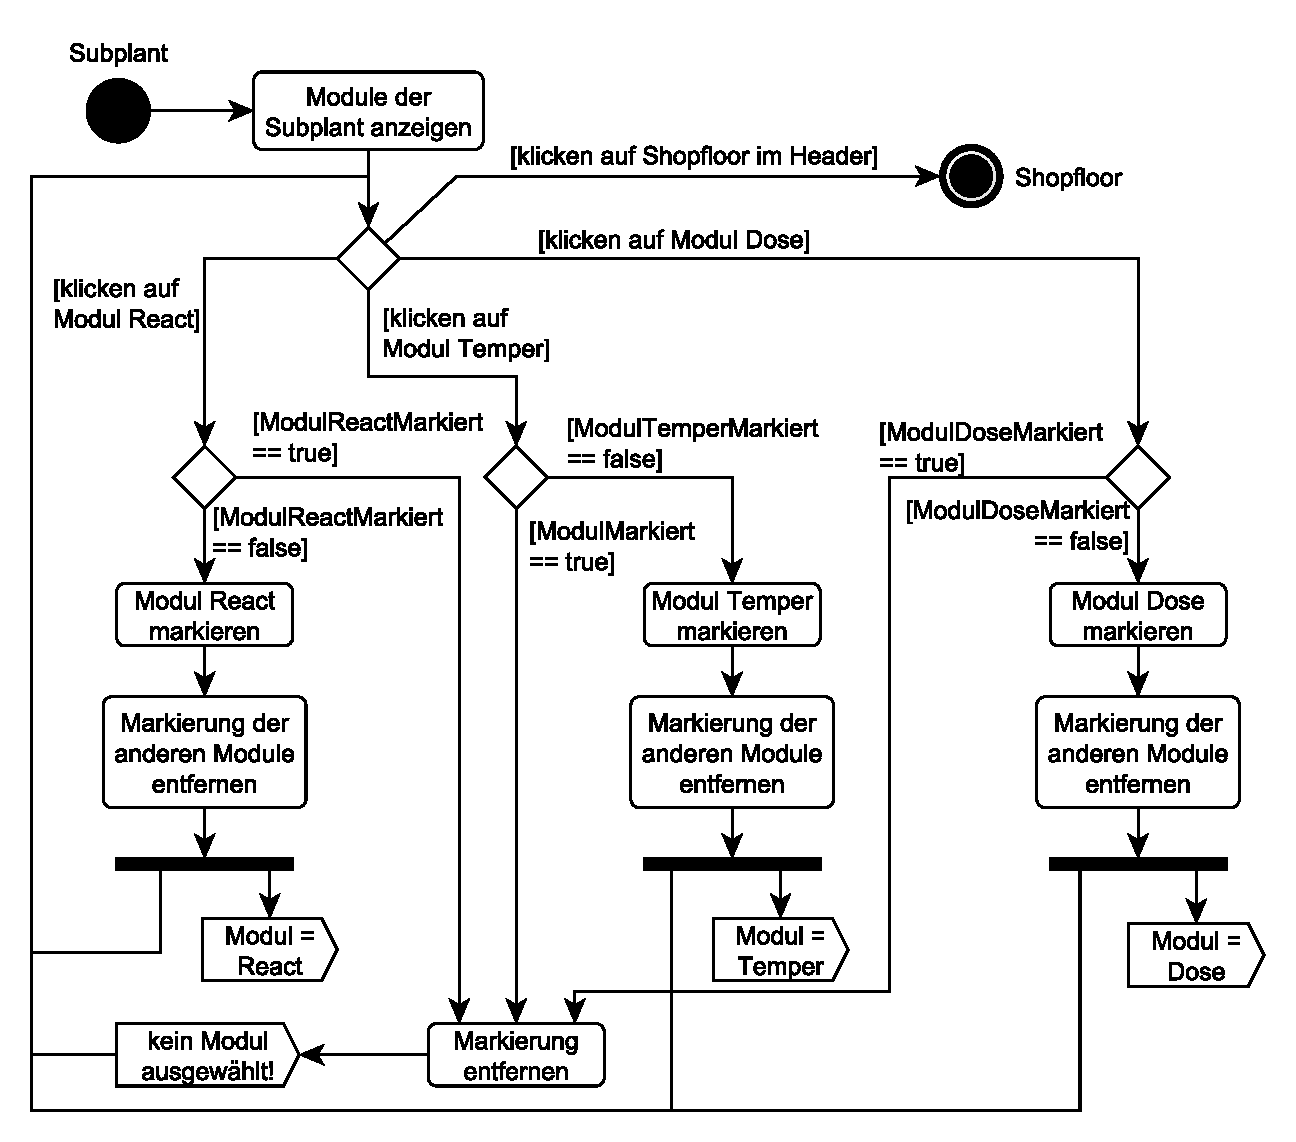
\includegraphics[scale=0.6]{DA_files/UML/Prototyp/Aktivitaetsdiagramm-Navigation-Module.pdf}
\caption{Aktivitätsdiagramm Navigation Subplant - Prototyp}
\label{pic:Aktivitaetsdiagramm-Navigation-Subplant}
\end{figure}

\subsection{Rezept}
Das Rezept zeigt entweder die Phases, die Procedures oder die Steps an. Ein Wechsel zwischen diesen Ansichten kann zum einen durch die Navigation ausgelöst werden. Zum anderen hat der Nutzer die Möglichkeit durch Klicken auf die einzelnen Phases und Procedurs den angezeigten Detailgrad des Rezepts zu verändern (siehe Abbildung \ref{pic:Zustandsdiagramm-Rezept}).
\begin{figure}[htbp]
\centering
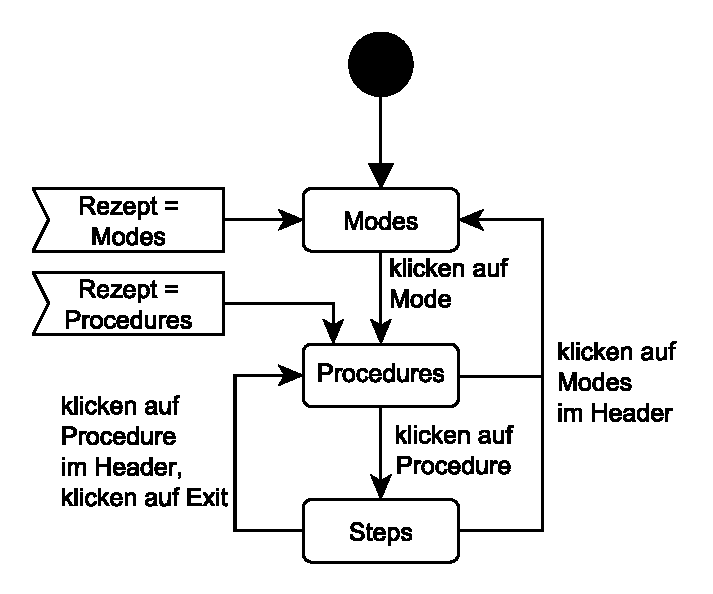
\includegraphics[scale=0.6]{DA_files/UML/Prototyp/Zustandsdiagramm-Rezept.pdf}
\caption{Zustandsdiagramm Rezept - Prototyp}
\label{pic:Zustandsdiagramm-Rezept}
\end{figure}
Innerhalb der verschiedenen Zustände des Rezepts sind weitere Interaktionen möglich. In den Procedures wird das angewählte Modul hervorgehoben (siehe Abbildung \ref{pic:Aktivitaetsdiagramm-Rezept-Procedures}). Bei den Steps ist es möglich durch Hoverfunktionen weitere Informationen zu erhalten (siehe Abbildung \ref{pic:Aktivitaetsdiagramm-Rezept-Steps}).
\begin{figure}[htbp]
\centering
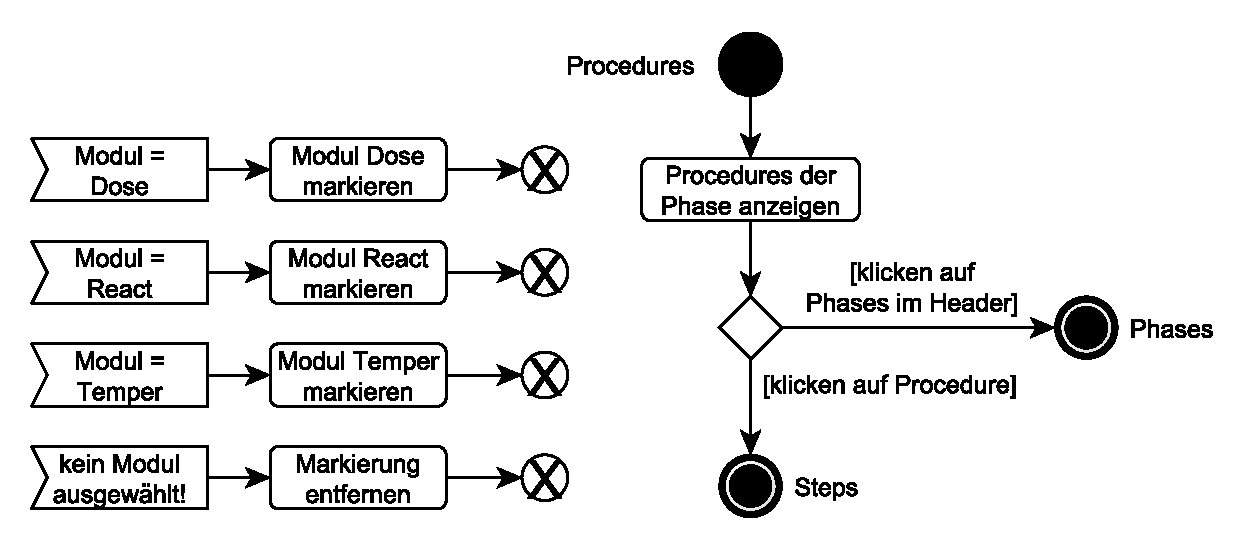
\includegraphics[scale=0.6]{DA_files/UML/Prototyp/Aktivitaetsdiagramm-Rezept-Procedures.pdf}
\caption{Aktivitätsdiagramm Rezept Procedures - Prototyp}
\label{pic:Aktivitaetsdiagramm-Rezept-Procedures}
\end{figure}

\begin{figure}[htbp]
\centering
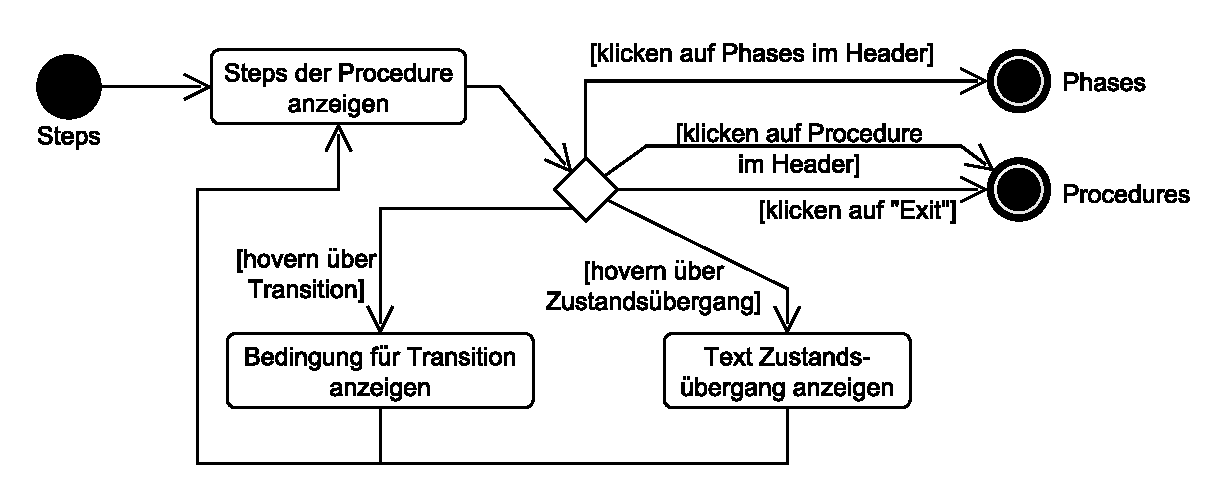
\includegraphics[scale=0.6]{DA_files/UML/Prototyp/Aktivitaetsdiagramm-Rezept-Steps.pdf}
\caption{Aktivitätsdiagramm Rezept Steps - Prototyp}
\label{pic:Aktivitaetsdiagramm-Rezept-Steps}
\end{figure}

\subsection{Service Launcher}
Der Service Launcher zeigt, abhängig von der gewählten Sortierung und dem ausgewählten Modul, in der Navigation die Services an (siehe Abbildung \ref{pic:Aktivitaetsdiagramm-ServiceLauncher}). Der Nutzer hat zudem die Möglichkeit durch Klicken auf den Service weitere Informationen zu bekommen. Es werden die möglichen Zustandsübergänge, der Operation Mode und die Strategy angezeigt (siehe Bild \ref{pic:Service-offen} \todo{ Quelle}). Ebenso kann der Nutzer durch Klicken auf das Zahnrad-Symbol die Einstellung der Parameter, der Strategy und des Operation Mode ändern. Solange ein Service ausgewählt ist, werden die anderen ausgeblendet und sind erst wieder anwählbar, wenn der aktuelle Service geschlossen wurde.
\begin{figure}[htbp]
\centering
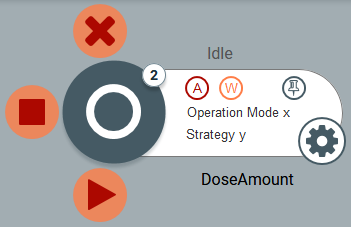
\includegraphics[scale=0.7]{DA_files/Bilder/Prototyp/Service-offen.png}
\caption{Angeklickter  Service}
\label{pic:Service-offen}
\end{figure}

\section{Problembeschreibung}
\label{5:Problembeschreibung}
Im Konzept sind bereits die Funktionalitäten für die Problembeschreibung erläutert. Im Rahmen des Prototypen sind diese konkret umgesetzt. Der Nutzer hat die Möglichkeit ein weiteres Ziel nicht nur hinzuzufügen, sondern auch wieder zu löschen. Zudem ist das Ziel Stillstandzeit editierbar. Die Veränderung der Ziele hat einen Einfluss auf die Lösungen, welche in Abschnitt \ref{5:Loesungen} näher spezifiziert sind. Keinen Einfluss hat in diesem Beispiel die Veränderung im Dropdown-Menü. Möchte der Nutzer sich die Lösungen ansehen, bringt ihn der Button \textbf{Lösungen finden} dort hin. Wie das Assistenzssystem auf die Interaktionen des Nutzers reagiert ist in Abbildung \ref{pic:Aktivitaetsdiagramm-Problem} dargestellt.

\begin{figure}[htbp]
\centering
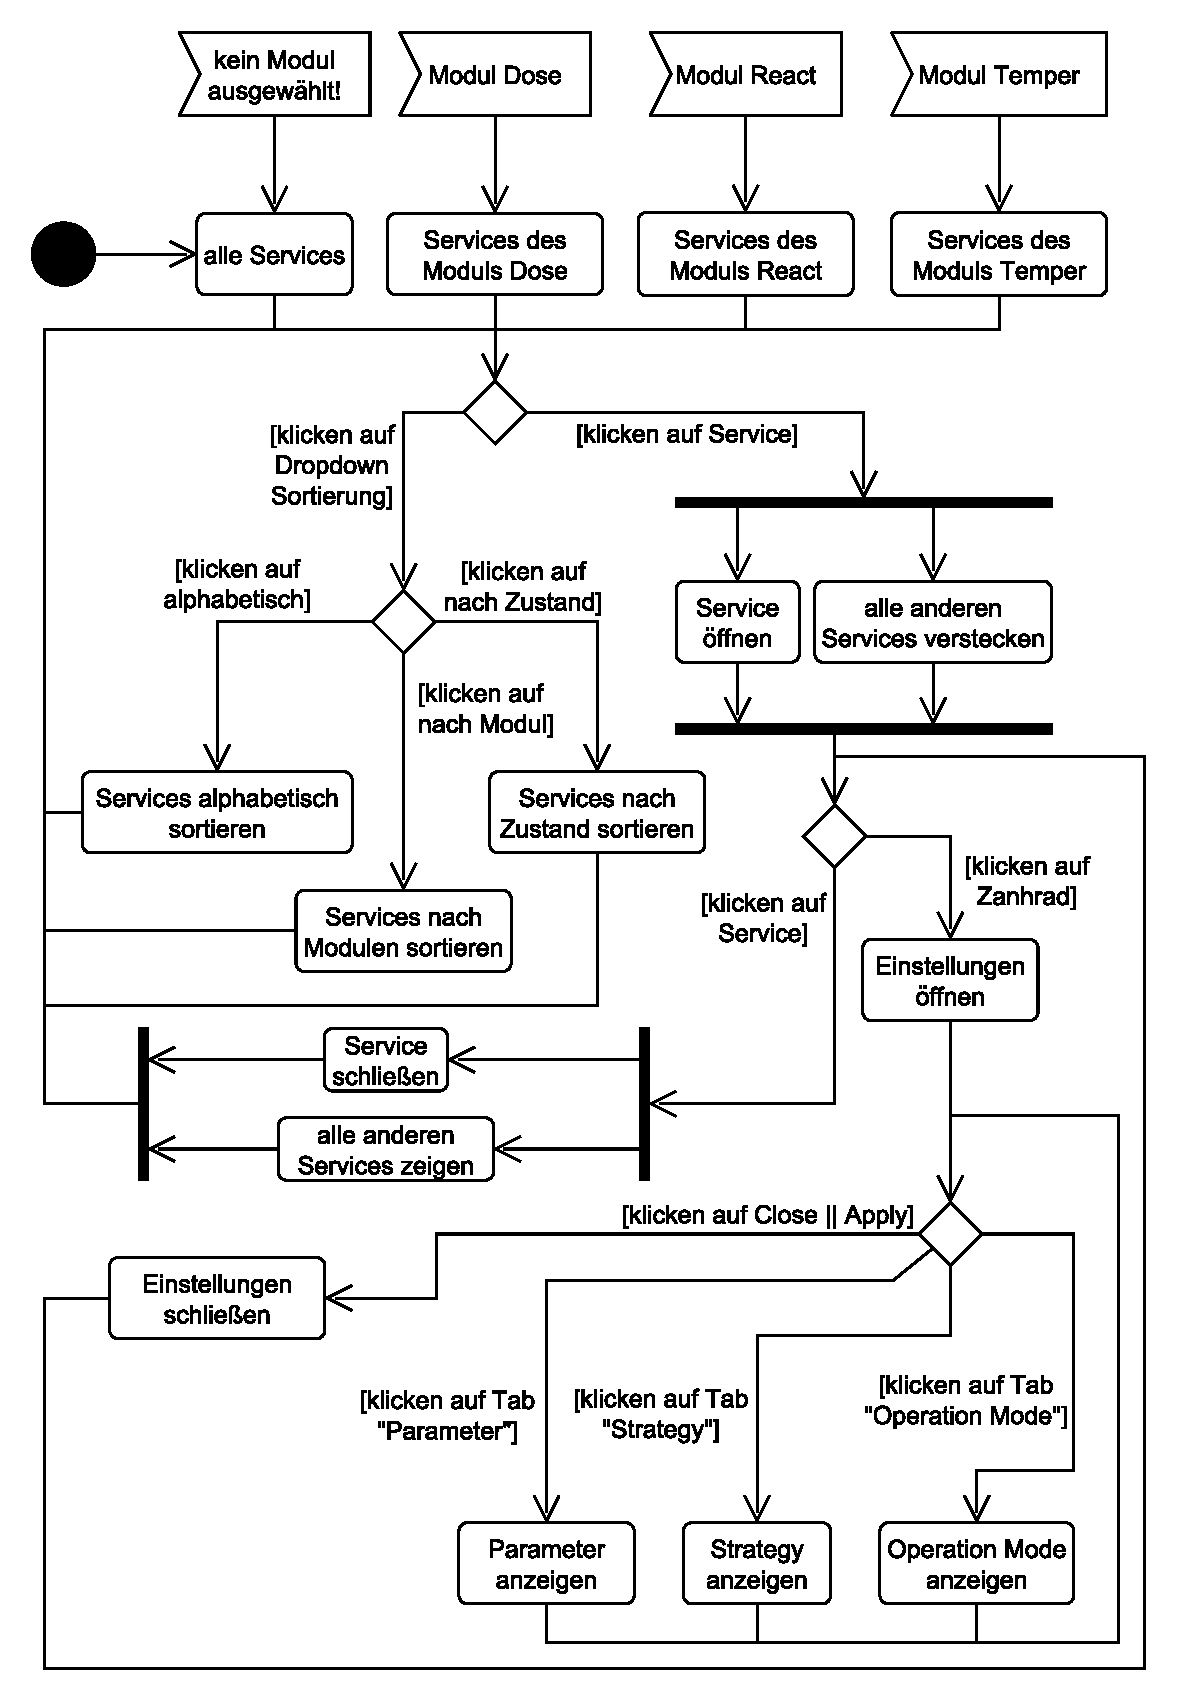
\includegraphics[scale=0.65]{DA_files/UML/Prototyp/Aktivitaetsdiagramm-ServiceLauchner.pdf}
\caption{Aktivitätsdiagramm Service Launcher - Prototyp}
\label{pic:Aktivitaetsdiagramm-ServiceLauncher}
\end{figure}

\begin{figure}[tbp]
\centering
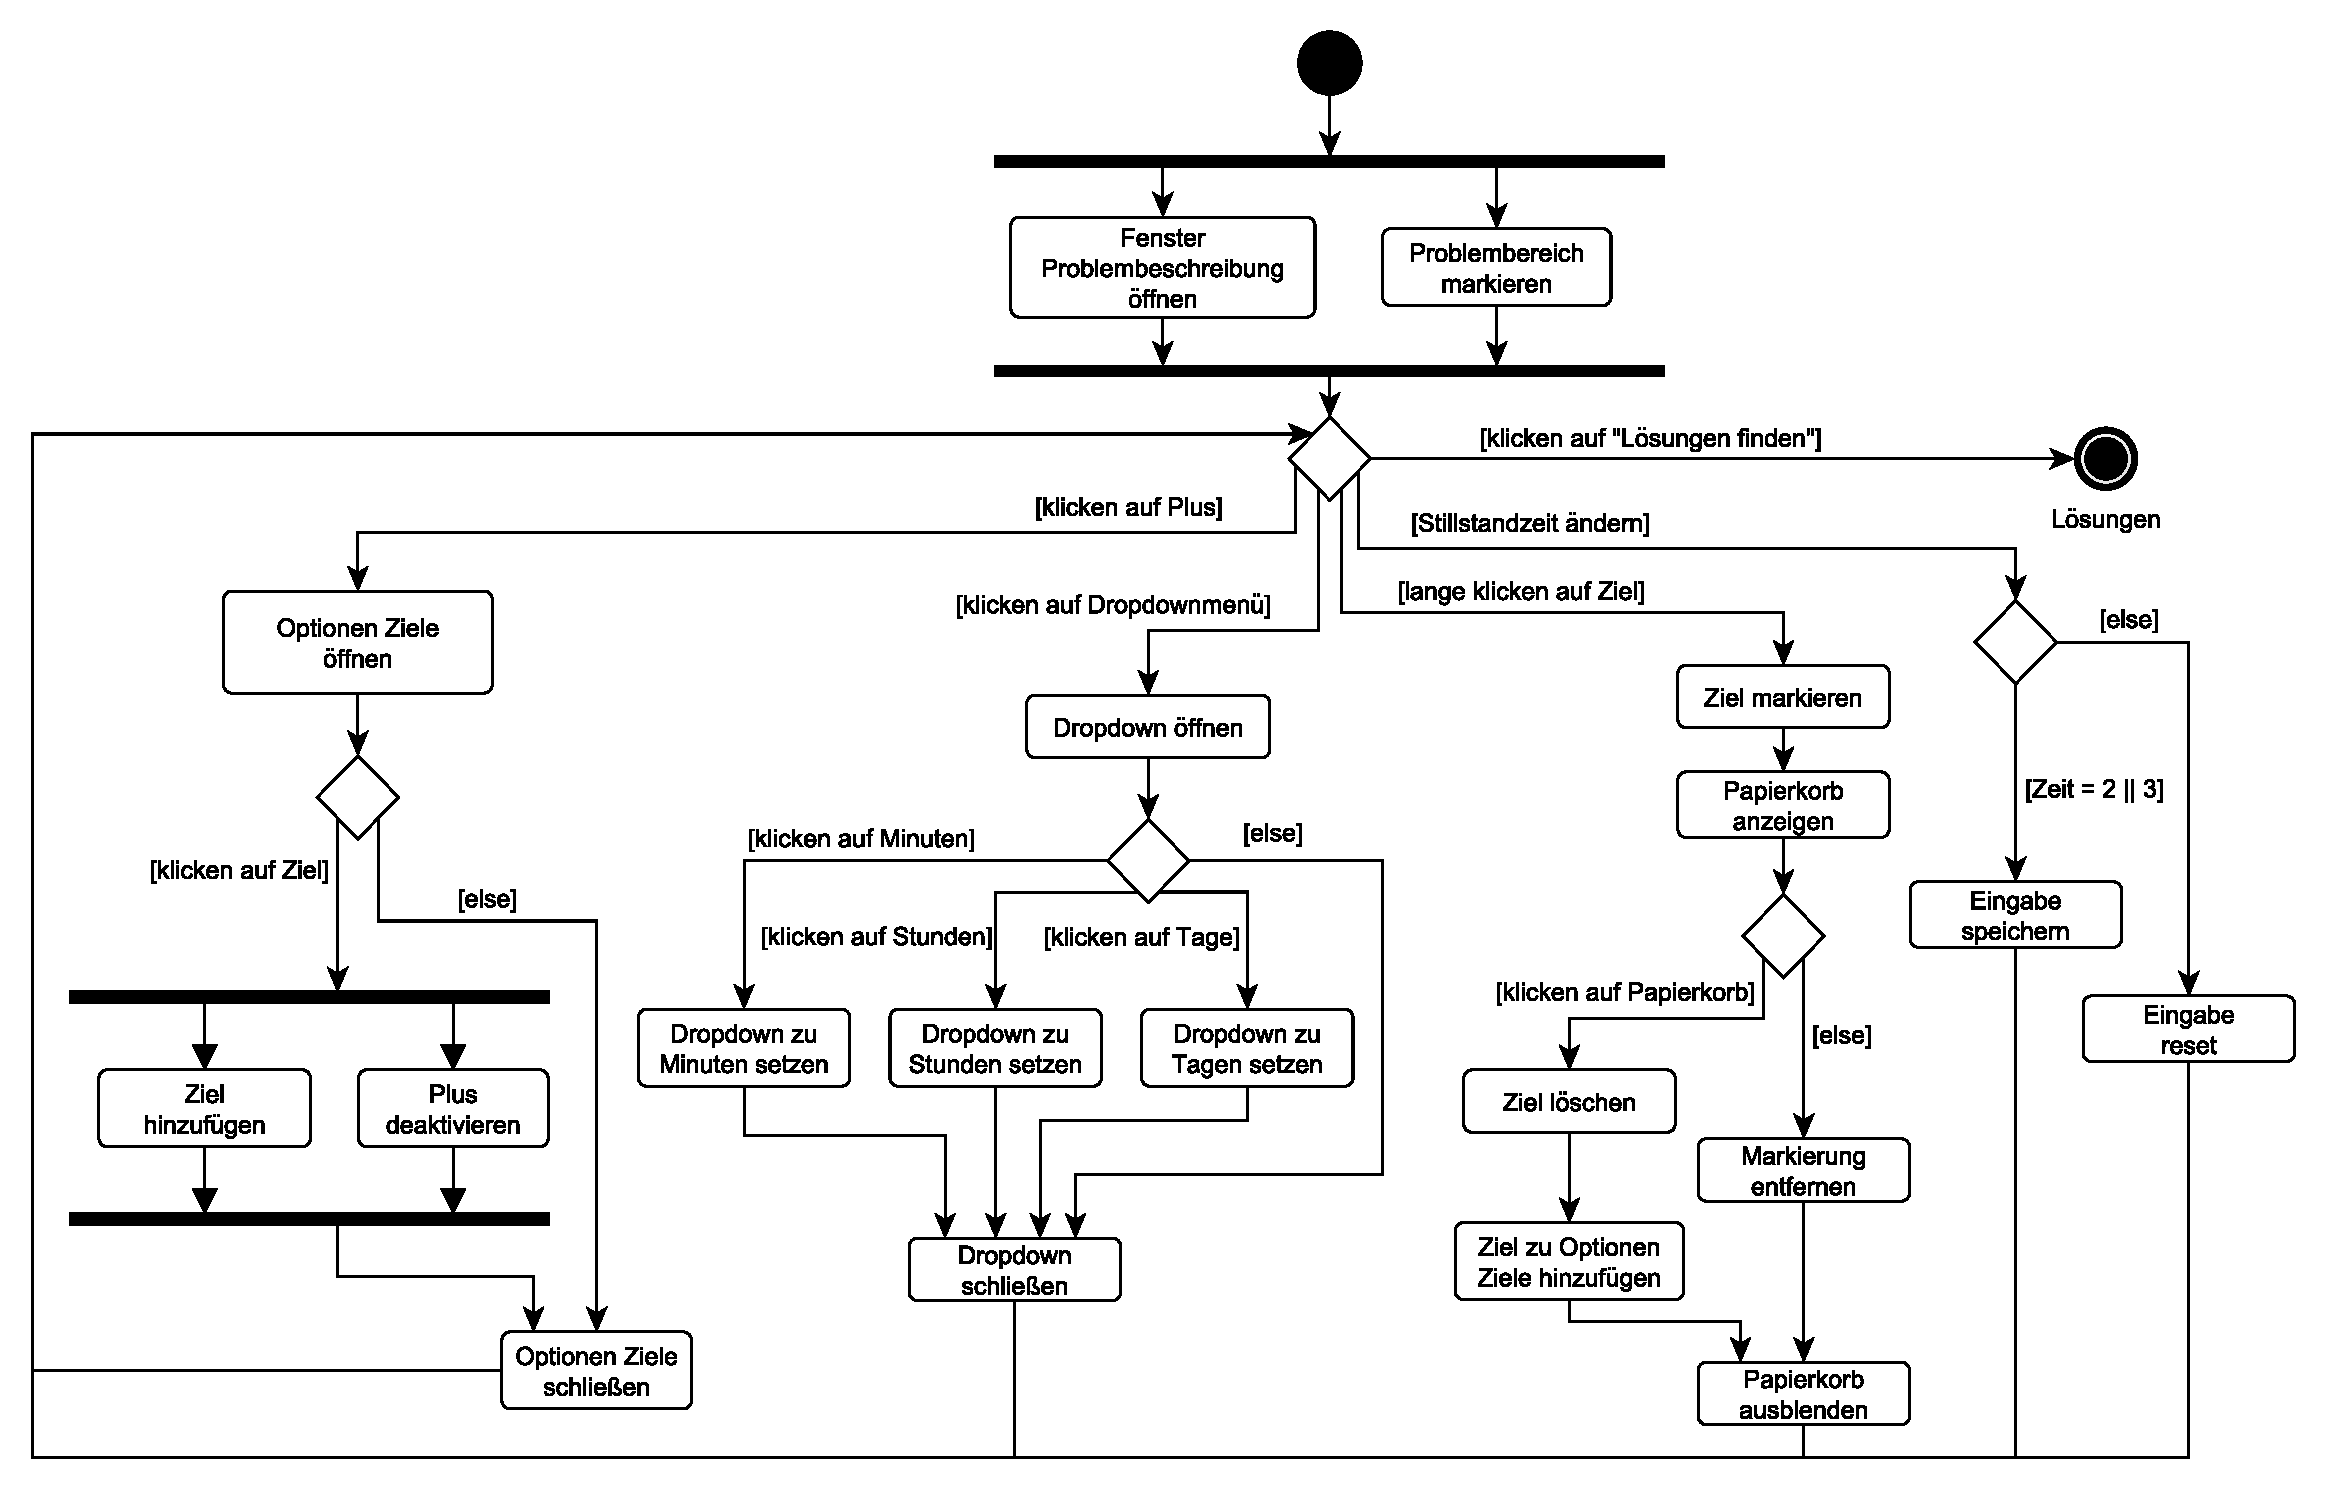
\includegraphics[angle=90,scale=0.5]{DA_files/UML/Prototyp/Aktivitaetsdiagramm-Problem.pdf}
\caption{Aktivitätsdiagramm Zustand Problem - Prototyp}
\label{pic:Aktivitaetsdiagramm-Problem}
\end{figure}

\section{Lösungen}
\label{5:Loesungen}
Die präsentierten Lösungen des Assistenzsystems orientieren sich an den eingegebenen Zielen des Nutzers. Der Nutzer hat die Möglichkeit durch Anwählen einer Lösung, die Veränderung in der Navigation, dem Rezept und dem Service Launcher anzusehen. Wie das Assistenzsystem auf die Auswahl des Nutzer reagiert, ist in Abbildung \ref{pic:Aktivitaetsdiagramm-Loesungen} dargestellt. Die Interaktionsmöglichkeiten der Prozessführungsebene verändern sich dabei nicht.

\begin{figure}[htbp]
\centering
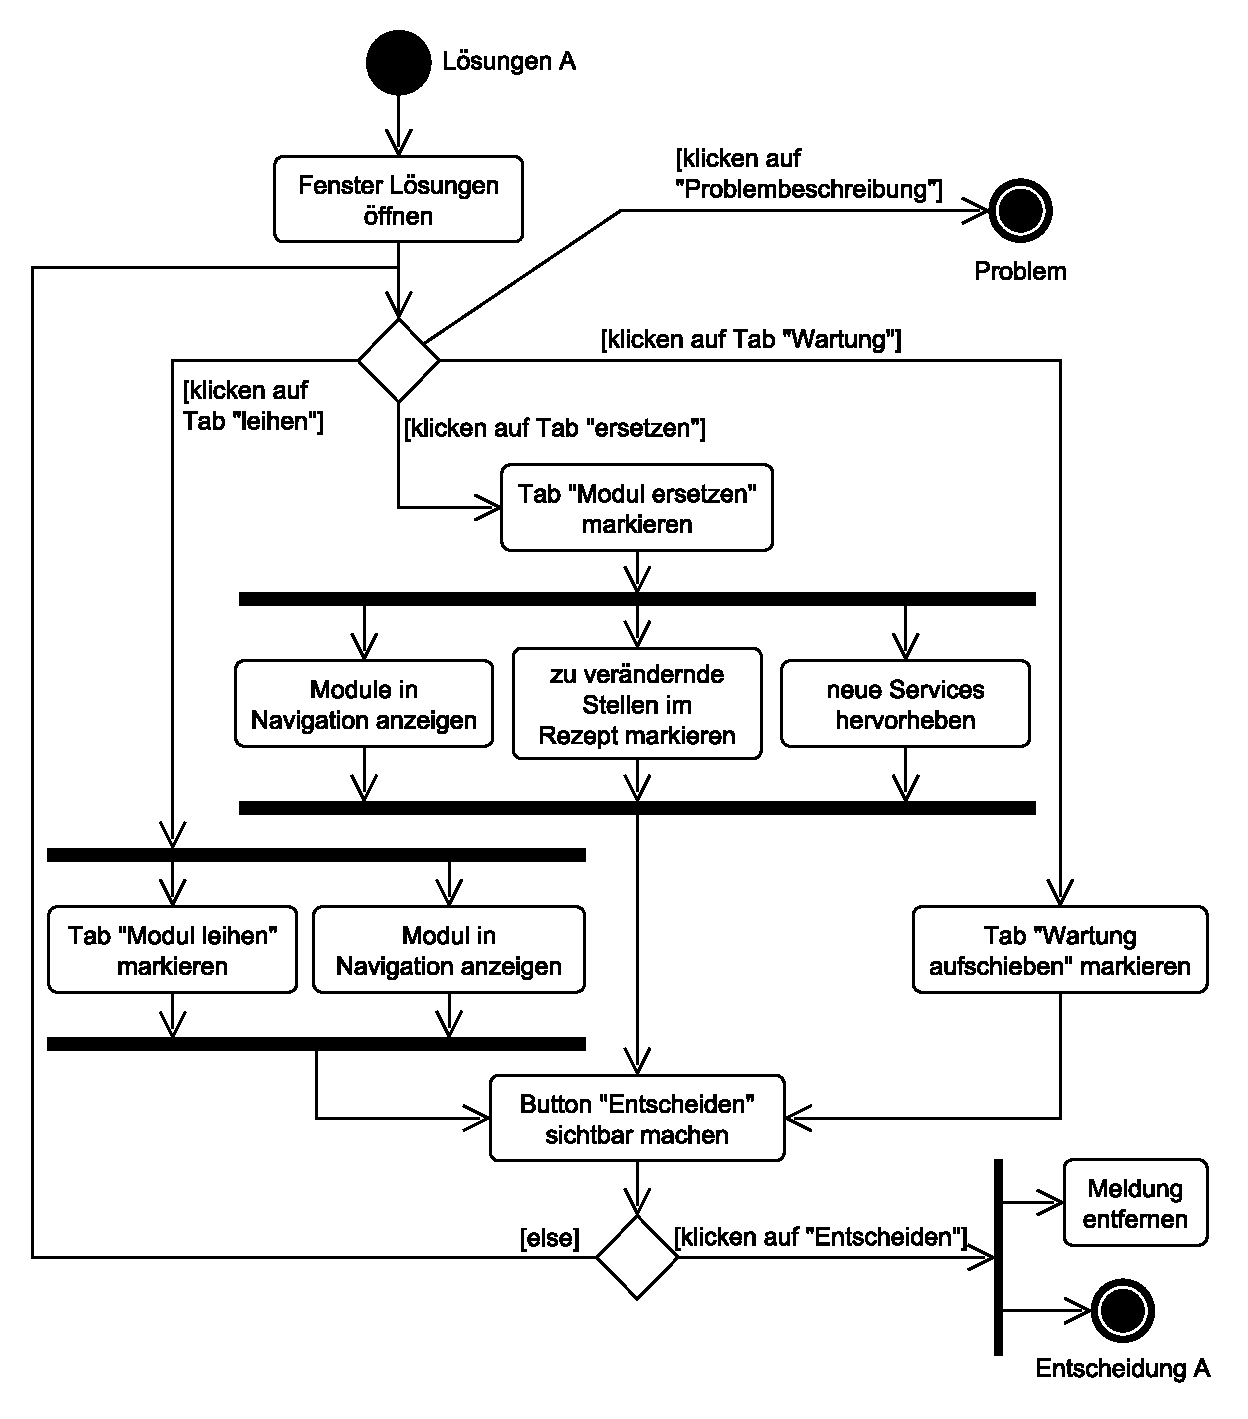
\includegraphics[scale=0.6]{DA_files/UML/Prototyp/Aktivitaetsdiagramm-Loesungen.pdf}
\caption{Aktivitätsdiagramm Lösungen - Prototyp}
\label{pic:Aktivitaetsdiagramm-Loesungen}
\end{figure}